
\section{Análise Estatística}

Um modelo de regressão linear generalizado para a distribuição de Poisson foi
proposto. Como o modelo considera apenas as contagens simuladas e a sequência
dos dados, o resultado da regressão é o valor da média (figura
\ref{Figure051-FailureSequence}).

\begin{center}
  $\langle\hat{y}\rangle = 4,9987$.
\end{center}

A elaboração de um histograma de frequência do número de falhas com a
distribuição ajustada auxilia a avaliação do modelo linear generalizado
(figura \ref{Figure052-FailureHistogram}).

\begin{center}
  $\hat{\lambda}=4,9987$.
\end{center}

Se aumentarmos o número de execuções simuladas e a probabilidade de se existir
aresta entre dois vértices quaisquer, é natural esperar que a média dos valores
preditos para o modelo considerado e o parâmetro Poisson estimado se aproximarão
do parâmetro Poisson utilizado para a simulação:

\begin{center}
  $\langle\hat{y_i}\rangle \longrightarrow \lambda \quad$ e $\quad \hat{\lambda}
  \longrightarrow \lambda$,
\end{center}

\noindent o que corrobora com a ideia de que quanto maior a amostra, melhor o
ajuste.

{
  \centering
  \captionsetup{type=figure}
	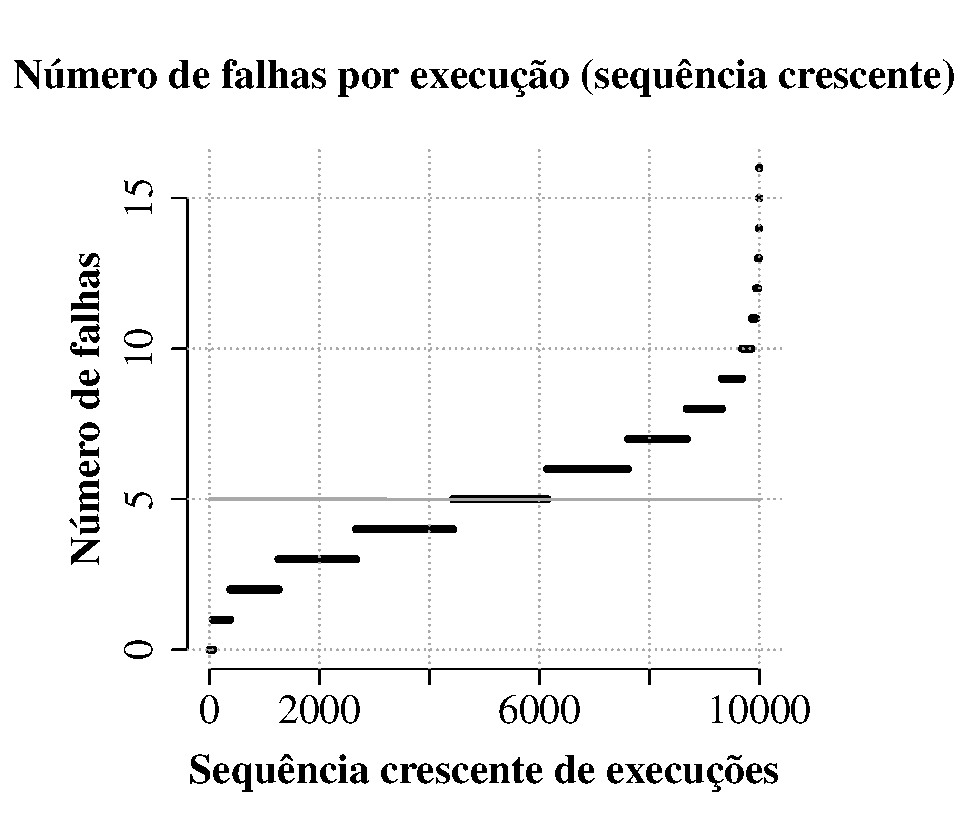
\includegraphics[scale=0.45]{./figures/Figure051-FailureSequence.pdf}
  \captionof{figure}{
    número de falhas por execução (de preto), em ordem crescente, e pontos
    ajustados pela regressão (de cinza). Média amostral para valor predito pelo
    modelo linear generalizado proposto: $\langle\hat{y}\rangle = 4,9987$.
  }
	\label{Figure051-FailureSequence}
}

{
  \centering
  \captionsetup{type=figure}
	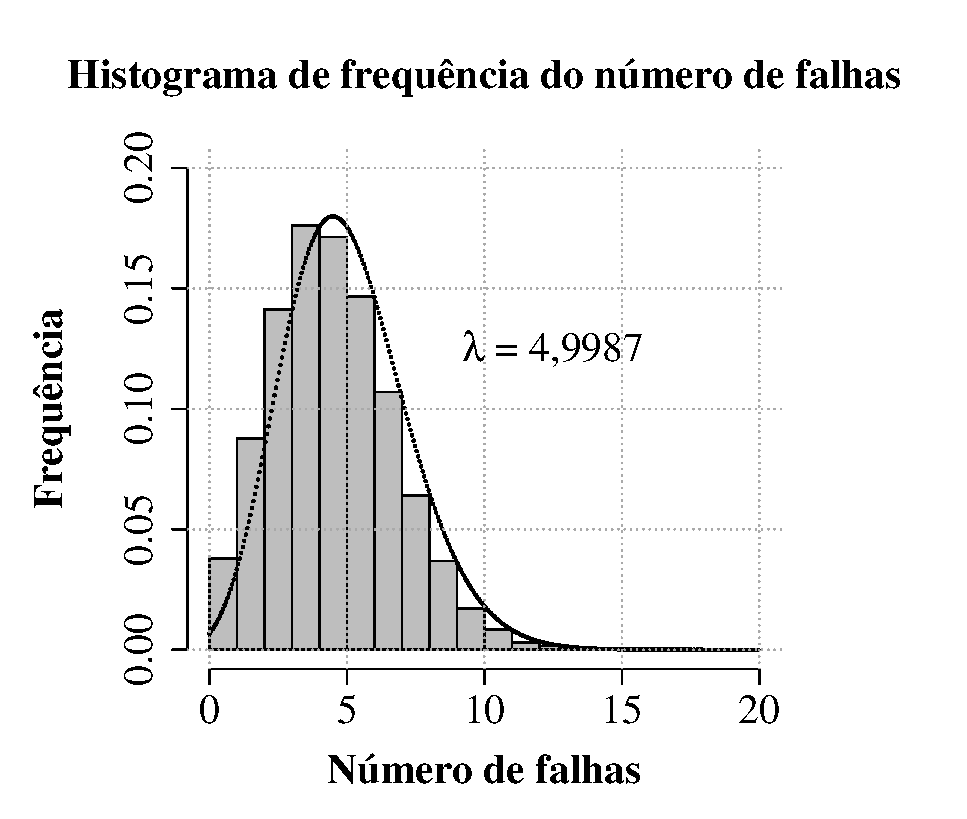
\includegraphics[scale=0.45]{./figures/Figure052-FailureHistogram.pdf}
  \captionof{figure}{
    histograma de frequência do número de falhas e pontos da distribuição de
    Poisson ajustada, onde $\hat{\lambda}=4,9987$.
  }
	\label{Figure052-FailureHistogram}
}

% exibir resultados

% analisar resultados
